\documentclass[tikz,border=8pt]{standalone}
\usepackage[T1]{fontenc}
\usepackage[utf8]{inputenc}
\usepackage{lmodern}
\usepackage{xcolor}
\usetikzlibrary{arrows.meta,positioning}

\definecolor{Ink}{HTML}{23385E}
\definecolor{Accent}{HTML}{1E6277}
\definecolor{Teal}{HTML}{2E9D8F}
\definecolor{Warm}{HTML}{E9754A}
\definecolor{Slate}{HTML}{66788E}
\definecolor{SoftBlue}{HTML}{D8ECF6}
\definecolor{SoftGreen}{HTML}{DDF5E9}
\definecolor{SoftOrange}{HTML}{FDE6D8}

\begin{document}
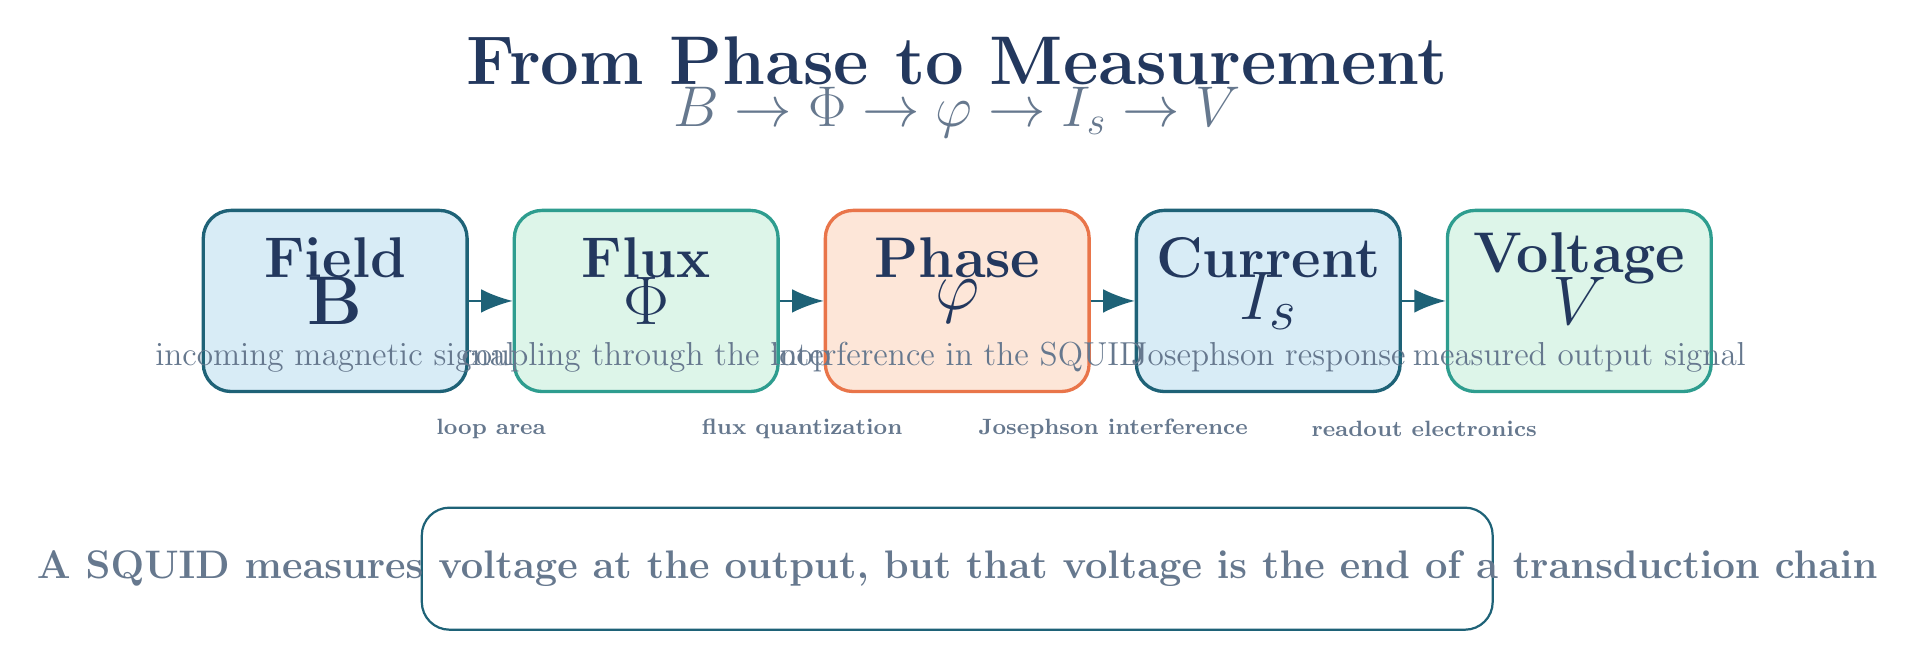
\begin{tikzpicture}[x=1cm,y=1cm,>=Latex]
  \tikzset{
    stage/.style={
      rounded corners=10pt,
      very thick,
      minimum width=3.35cm,
      minimum height=2.3cm,
      align=center,
      inner sep=6pt,
      text=Ink
    },
    stageblue/.style={stage, draw=Accent, fill=SoftBlue},
    stagegreen/.style={stage, draw=Teal, fill=SoftGreen},
    stageorange/.style={stage, draw=Warm, fill=SoftOrange},
    flow/.style={-{Latex[length=4mm,width=3mm]}, thick, Accent},
    flowlabel/.style={font=\bfseries\footnotesize, text=Slate},
    boxtitle/.style={font=\bfseries\fontsize{22}{24}\selectfont, text=Ink},
    boxsymbol/.style={font=\bfseries\fontsize{30}{32}\selectfont, text=Ink},
    boxsub/.style={font=\fontsize{12}{14}\selectfont, text=Slate},
    headtitle/.style={font=\bfseries\fontsize{24}{26}\selectfont, text=Ink},
    headformula/.style={font=\bfseries\fontsize{20}{22}\selectfont, text=Slate},
    note/.style={font=\bfseries\fontsize{15}{17}\selectfont, text=Slate}
  }

  \node[headtitle] at (10.0,7.6) {From Phase to Measurement};
  \node[headformula] at (10.0,6.95) {$B \rightarrow \Phi \rightarrow \varphi \rightarrow I_s \rightarrow V$};

  \node[stageblue]   (field)   at (2.1,4.55) {};
  \node[stagegreen]  (flux)    at (6.05,4.55) {};
  \node[stageorange] (phase)   at (10.0,4.55) {};
  \node[stageblue]   (current) at (13.95,4.55) {};
  \node[stagegreen]  (voltage) at (17.9,4.55) {};

  \node[boxtitle] at (field.center) [yshift=0.55cm] {Field};
  \node[boxsymbol] at (field.center) {B};
  \node[boxsub] at (field.center) [yshift=-0.72cm] {incoming magnetic signal};

  \node[boxtitle] at (flux.center) [yshift=0.55cm] {Flux};
  \node[boxsymbol] at (flux.center) {${\Phi}$};
  \node[boxsub] at (flux.center) [yshift=-0.72cm] {coupling through the loop};

  \node[boxtitle] at (phase.center) [yshift=0.55cm] {Phase};
  \node[boxsymbol] at (phase.center) {${\varphi}$};
  \node[boxsub] at (phase.center) [yshift=-0.72cm] {interference in the SQUID};

  \node[boxtitle] at (current.center) [yshift=0.55cm] {Current};
  \node[boxsymbol] at (current.center) {$I_s$};
  \node[boxsub] at (current.center) [yshift=-0.72cm] {Josephson response};

  \node[boxtitle] at (voltage.center) [yshift=0.55cm] {Voltage};
  \node[boxsymbol] at (voltage.center) {$V$};
  \node[boxsub] at (voltage.center) [yshift=-0.72cm] {measured output signal};

  \draw[flow] (field.east) -- (flux.west);
  \draw[flow] (flux.east) -- (phase.west);
  \draw[flow] (phase.east) -- (current.west);
  \draw[flow] (current.east) -- (voltage.west);

  \node[flowlabel] at (4.08,2.92) {loop area};
  \node[flowlabel] at (8.03,2.92) {flux quantization};
  \node[flowlabel] at (11.98,2.92) {Josephson interference};
  \node[flowlabel] at (15.93,2.92) {readout electronics};

  \node[
    rounded corners=10pt,
    draw=Accent,
    thick,
    fill=white,
    minimum width=13.6cm,
    minimum height=1.55cm,
    align=center,
    inner sep=7pt
  ] at (10.0,1.15) {};
  \node[note] at (10.0,1.15) {A SQUID measures voltage at the output, but that voltage is the end of a transduction chain};
\end{tikzpicture}
\end{document}
